\documentclass [a4paper, 12pt] {article}

\usepackage {graphicx}
\usepackage{fullpage}

\begin{document}

\section{Gravitational Lensing Bias}

It is well known that the effect of gravitational lensing is a powerful tool, which can manageably be exploited to boost the magnification of intrinsically faint or very distant galaxies (see Section- grav lensing). However, it is now thought that the high incidence of gravitational lensing in high-redshift observations will distort flux and number density measurements of the earliest galaxies\cite{distortionsinthegravitationallens}. A recent study (Wyithe and Stuart 2011) makes the case that the Hubble Space Telescope's (HST) current view of these galaxies has been significantly altered by gravitational lensing. Moreover, any planned galaxy surveys in the future, such as those with the James Webb Space Telescope (JWST), need to be designed to account for these substantial lensing biases at these extreme distances\cite{wyithestuart2011}.

\subsection{Magnification Bias}
Along a random line of sight, the light from distant source objects may be distorted- appearing brighter or being fragmented, so it is observed as multiple images- due to gravitational lensing by galaxies in the foreground. The raw probability of multiple imaging for high-redshift objects is ~0.5\%. However, the statistics can potentially become skewed by far greater amounts owing to something known as \emph{magnification bias}. Essentially, this is the magnification of intrinsically faint galaxies- that otherwise would be undetectable- to observed fluxes above the limit for a particular survey, leading to an excess of lensed galaxies among flux-limited samples. This magnification bias is expected to be significant at $z>8$. This would mean, for example, that if in an observation at $z>10$ there existed only a few galaxies above the detection limits, this number could be boosted by an order of magnitude, so that 10-30 galaxies were actually observed\cite{Cosmicmagnifyinglenses}. Consequently, gravitational lensing will likely dominate the observed properties of such early galaxies.
\\
\newline
The study, mentioned above, assesses the magnification bias among high-redshift galaxies in the Hubble Ultra-Deep Field (HUDF) by calculating the fraction of galaxies above the magnitude limit which will have been multiply imaged. They predict that at $z\approx6-7$, ~1\% of galaxies will be lensed; at $z\approx8-10$ this fraction can increase to up to a few tens of percent\cite{wyithestuart2011}. It should be noted that these values are subject to increasing sensitivity, at higher redshifts, to the true value of the characteristic magnitude M* (see section-Schechter function?)- as the survey limit may get much closer to M*, whose value is still highly uncertain. This sensitivity is illustrated in~Figure \ref{fig:gravhst1}, with the fraction of multiply lensed galaxies, $F_{mult}$, expected to be seen at different redshifts. One can clearly see that gravitational lensing biases become more of an issue the higher the redshift being observed.
\\
\newline
The corresponding graph in~Figure \ref{fig:gravjwst1} gives some idea of how this factor will continue to be an issue as telescopes with increased optical depth and resolution, such as JWST, become operational. For the ultra-deep and medium deep surveys, a multiply imaged fraction higher than $F_{mult}\approx10\%$ could be observed at $z>12$ and $z>16$ respectively.
\\
\newline
The magnification bias will additionally cause an overconcentration of high-redshift galaxies around foreground clusters. This correlation could be considered as an alternative means of studying the effects of gravitational lensing. For the JWST, it is thought that the majority of galaxies at extreme redshifts ($z>14$) will be $<1~arcsec$ from a bright foreground galaxy, meaning they will have been gravitationally magnified into the sample- a startling prediction\cite{wyithestuart2011}.

\begin{figure}
\begin{center}
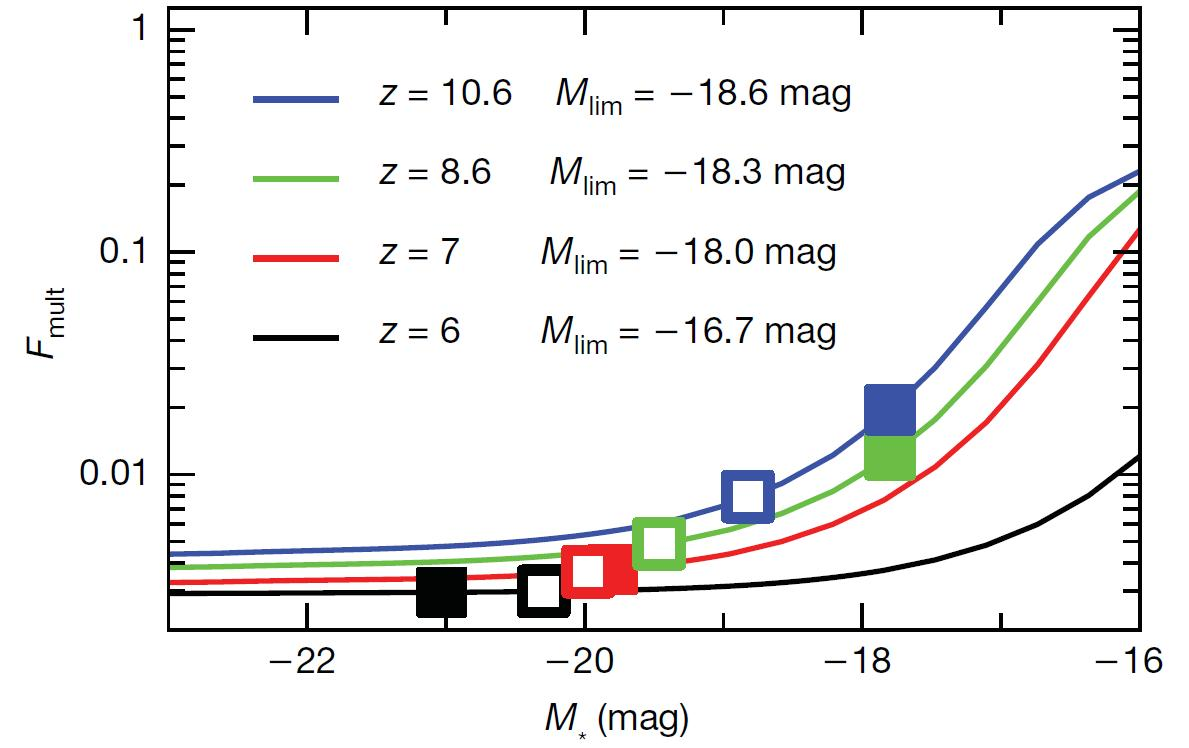
\includegraphics[scale=0.5]{gravhst1.jpg}
\end{center}
\caption{Graph showing the fraction of galaxies that are multiply imaged,  $F_{mult}$, at different redshifts, as a function of the characteristic magnitude, M*, for the HST. The closed and open squares represent alternative estimates of M*.}\label{fig:gravhst1}
\end{figure}

\begin{figure}
\begin{center}
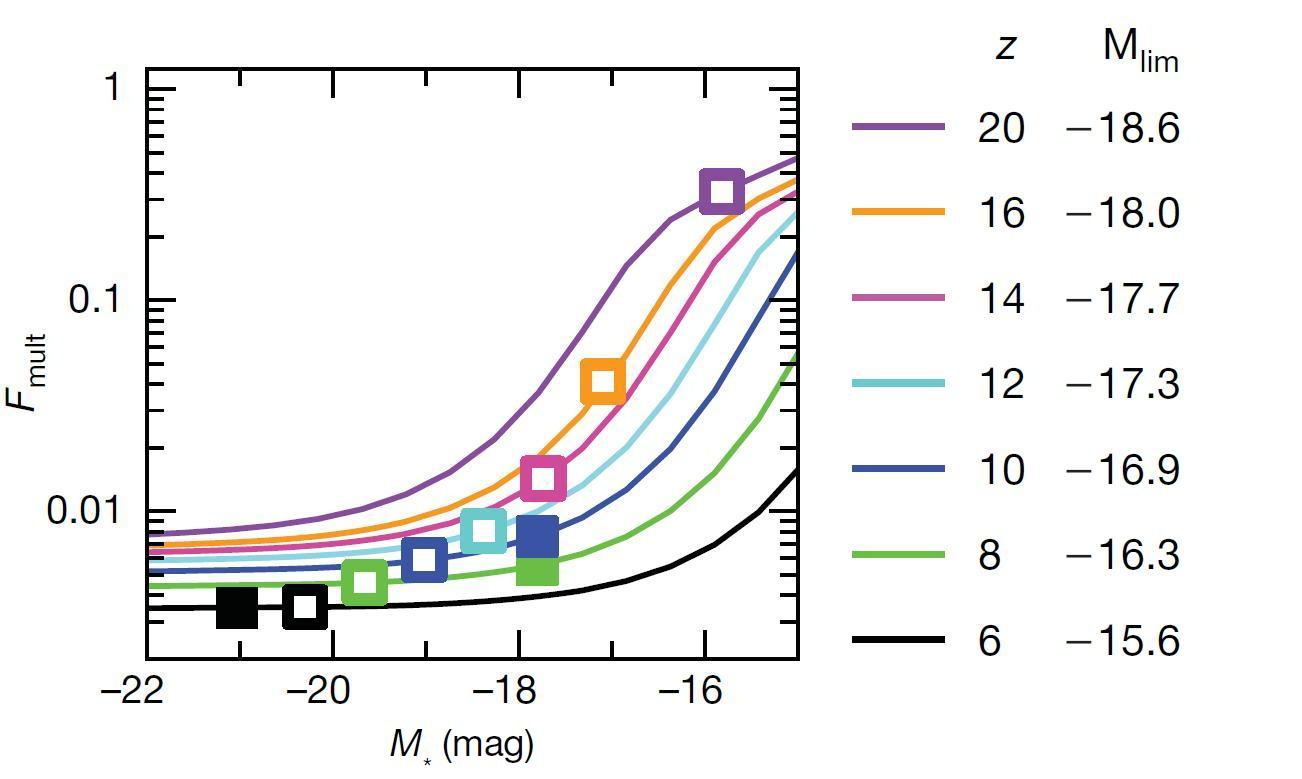
\includegraphics[scale=0.5]{gravjwst1.jpg}
\end{center}
\caption{Graph showing the fraction of multiply imaged galaxies against M* at different redshifts, for the JWST ultra-deep survey.}\label{fig:gravjwst1}
\end{figure}

\subsection{Effect on the Luminosity Function}

The distortion of galaxy number counts and their observed magnitudes brought about by the magnification bias will have a profound effect on the luminosity function, the properties of which, currently beyond $z\approx8$, are highly uncertain.~Figure \ref{fig:gravlumfun} illustrates the potential for the dramatic effect gravational lensing can have on the shape of the luminosity function.
\\
\newline
Current luminosity functions at $z>7$ are not corrected in any way for gravitational lensing. Any future studies will need to be prescribed with a detailed understanding of the magnification bias of high-redshift sources in order to discover the veritable unlensed shape of the luminosity function. However, allowing for the precise modelling of the involved biases, the exploitation of the correlation of high-z sources and foreground galaxies will be invaluable for probing the otherwise inaccessible shape of the luminosity function at these redshifts.

\begin{figure}
\begin{center}
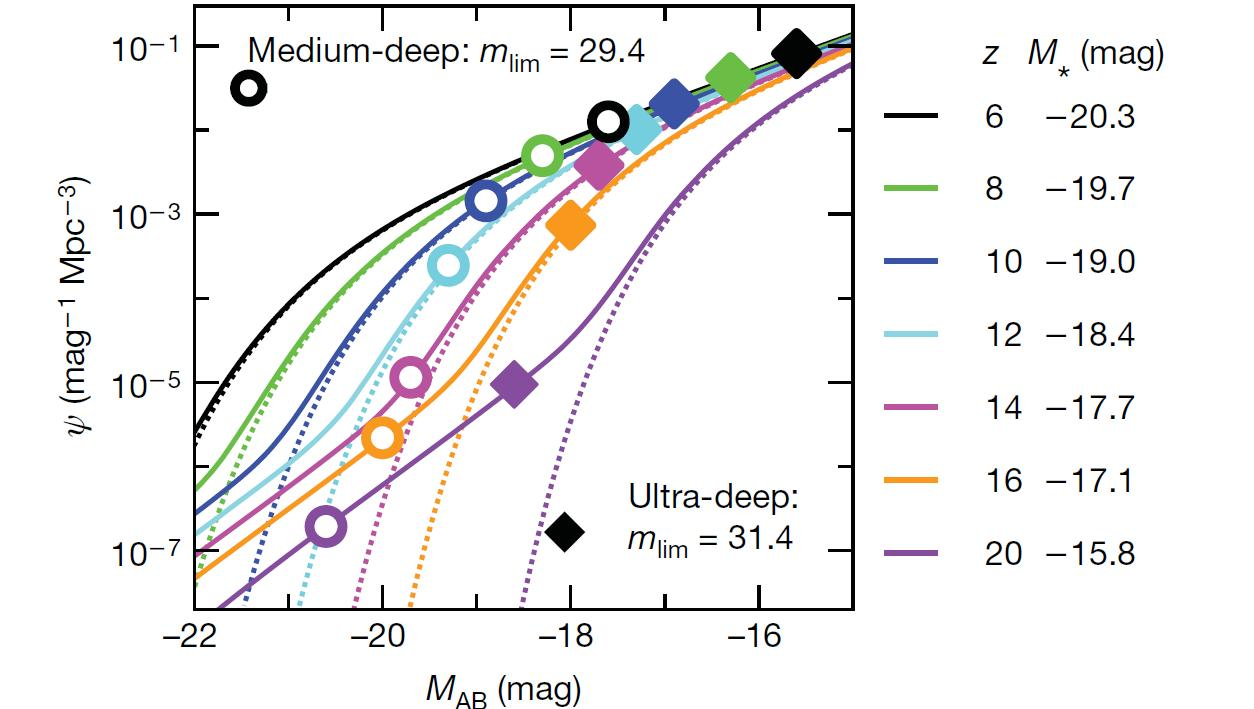
\includegraphics[scale=0.5]{gravlumfun.jpg}
\end{center}
\caption{Graph detailing the lens-induced distortion of the luminosity function. Dashed lines represent the unlensed shape, solid lines the modified shape due to gravitational lensing.}\label{fig:gravlumfun}
\end{figure}

\end{document}



 